\documentclass[12pt, 
openright, 
oneside, 
%twoside, %TCC: Se seu texto tem mais de 100 páginas, descomente esta linha e comente a anterior
a4paper,    
%english,   
brazil]{facom-ufu-abntex2}



\autor{Igor Batista Fernandes} 
\data{2018}
\orientador{Profa. Maria Adriana Vidigal de Lima} 
\titulo{Desenvolvimento de jogos 2D multiplataforma utilizando
OpenGL e Java} 

\begin{document}
\pagenumbering{arabic}
% ----------------------------------------------------------
% ELEMENTOS PRÉ-TEXTUAIS

\imprimircapa
\begin{folhadeaprovacao}

  \begin{center}
    {\ABNTEXchapterfont\large\imprimirautor}

    \vspace*{\fill}\vspace*{\fill}
    {\ABNTEXchapterfont\bfseries\Large\imprimirtitulo}
    \vspace*{\fill}
    
    \hspace{.45\textwidth}
    \begin{minipage}{.5\textwidth}
    \imprimirpreambulo
    \end{minipage}%
    \vspace*{\fill}
   \end{center}
    
   %Trabalho aprovado. 
   \imprimirlocal, XX de XX de 2018: %TCC:

   \assinatura{\textbf{\imprimirorientador} \\ Orientador}  
   \assinatura{\textbf{Professor}}% \\ Convidado 1} %TCC:
   \assinatura{\textbf{Professor}}% \\ Convidado 2} %TCC:
   %\assinatura{\textbf{Professor} \\ Convidado 3}
   %\assinatura{\textbf{Professor} \\ Convidado 4}
      
   \begin{center}
    \vspace*{0.5cm}
    {\large\imprimirlocal}
    \par
    {\large\imprimirdata}
    \vspace*{1cm}
  \end{center}
  
\end{folhadeaprovacao}
%-------------------------------------------
% RESUMO

\begin{resumo} 

Este trabalho propõe a criação de um jogo multiplataforma  para desktop intitulado Traveller.
A elicitação dos requisitos para a elaboração do jogo será documentada em um artefato denominado \textit{Game Design Document} que permite estruturar, sistematizar e organizar 
o processo de construção do jogo.
A implementação de código será realizada na linguagem Java e através da API gráfica OpenGL usando GLFW (OpenGL Frame Work). 
O jogo será elaborado utilizando-se algoritmos procedurais para geração de algumas artes e ambientes, algoritmos genéticos para o comportamento de Non Playable Characters (NPC) e padrões de projeto como o MVC.
 
 \vspace{\onelineskip}
 \noindent
 \textbf{Palavras-chave}: Indie Game, Game Design Document, Jogos, Java, OpenGL
\end{resumo}

\begin{abstract} 
This work proposes to develop a multiplataform game for desktop entitled Traveller. The elicitation of requisites for the game will be documented in an artifact called Game Design Document which allows to structure, systematize and organize the process of building a game. The code implementation will be done in Java through the API OpenGL and GLFW.  The game will be elaboreted using procedural algorithms to generate some art and environment, genetic algorithms for NPC behaviours and design patterns such as MVC.

 \vspace{\onelineskip}
    
 \noindent
 \textbf{Keywords}: Indie Game, Game Design Document, Games, Java, OpenGL %TCC:
\end{abstract}
\cleardoublepage

% ------------------------------------------
% LISTA DE FIGURAS

\pdfbookmark[0]{\listfigurename}{lof}
\listoffigures*
\cleardoublepage

% ------------------------------------------
% LISTA DE TABELAS

\pdfbookmark[0]{\listtablename}{lot}
\listoftables*
\cleardoublepage

% ------------------------------------------
% LISTA DE CÓDIGOS
\pdfbookmark[0]{\listtablename}{lol}
\lstlistoflistings
\cleardoublepage

% ------------------------------------------
% LISTA DE ABREVIATURAS OU SIGLAS

\begin{siglas} 
  \item[GDD] Game Design Document 
  \item[API] Application Programming Interface
  \item[MVC] Model-view-controller
  \item[OpenGL] Open Graphics Library
  \item[GPU] Graphics Processing Unit
  \item[GLFW] Graphics Library Framework
  \item[GLSL] OpenGL Shading Language
  \item[NPC] Non Playable Character
  \item[HUD] Heads-Up Display
  \item[ASD] A Ser Definido
  \item[FPS] Frames per second
  \item[px] Pixel (Unidade de medida)
  \item[VBO] Vertex Buffer Object
  \item[VAO] Vertex Array Object
\end{siglas}


% SUMÁRIO
% ---
\pdfbookmark[0]{\contentsname}{toc}
\tableofcontents*
\cleardoublepage


% ------------------------------------------
% COMEÇAR O TEXTO

%\textual

% ------------------------------------------% INTRODUÇÃO

% colocar como subitem 
%\chapter*[Introdução]{Introdução}
%\addcontentsline{toc}{chapter}{Introdução}

\chapter{Introdução}

\section{Visão Geral da Proposta}
O mercado internacional de jogos movimentará aproximadamente 108.9
bilhões de dólares distribuídos entre 2.2 bilhões de jogadores. Destes, 58\%
representam os segmentos de PC e consoles \cite{GameMarketArticle}. Além de ser uma área
comercial extremamente lucrativa é também interdisciplinar e aproxima
conceitos de Computação, Design gráfico, Música, Artes e outras esferas do
conhecimento.
Para a elaboração de um projeto bem construído e com alto potencial de
sucesso é necessário respeitar as etapas de pré-produção, produção, testes
e pós-produção. Ao longo de todas as etapas serão definidas estratégias de
implementação em linguagens orientadas a objetos, Engenharia de software
voltada par jogos e metodologias ágeis.
Desenvolvida pela Khronos Group a API OpenGL fornece tudo que há de mais
avançado em aplicações gráficas, sendo acelerada diretamente em
hardware, multiplataforma, robusta e totalmente escalável.


%Objetivo
\section{Objetivo}
O objetivo é desenvolver um jogo seguindo a construção de um Game Design
Document (GDD) e ter o produto final publicado e distribuído
comercialmente de maneira digital. Ao final deste documento será
apresentada a primeira fase do capítulo introdutório, jogável e com
qualidade profissional.

\section{Justificativa e Motivação}
O consumo cada vez maior deste tipo de produto pela população de todas as idades traz cada vez mais oportunidades de trabalho e aprendizagem.
A insuficiência de materiais em língua portuguesa sobre os processos de desenvolvimento e planejamento de jogos é um grande instigador desse trabalho. Neste contexto, esse trabalho aborda todas as etapas pelas quais um jogo passa para torna-se um software que será distribuído e jogado por pessoas do mundo todo.


\section{Metodologia}


Este trabalho se classifica como uma pesquisa aplicada, sendo o método de desenvolvimento baseado nas etapas a seguir:

Etapa 1 – Revisão sistemática em desenvolvimento de jogos
\begin{itemize}
\item Desenvolvimento de Jogos estilo RPG - levantamento bibliográfico, identificação e organização dos trabalhos relacionados e do estado da arte;
\item Pesquisa documental sobre engenharia de software e padrões de projeto aplicada a jogos;
\item Pesquisa documental sobre o uso de metodologias ágeis no desenvolvimento de jogos.
\end{itemize}

Etapa 2 – Projeto do jogo identificando os conceitos a serem aplicados 
\begin{enumerate}
\item Pré-Projeto: análise de mercado, tendências e viabilidade;
definição da ideia do seu jogo; atividades a serem realizadas;
equipe.
\item Pré-Produção: elaboração do Game Design Document, elaboração do Roteiro, elaboração do Documento de Arte e Design Gráfico; criação de protótipos para testar ideias, mecânicas e conceitos;
\item Plano de Produção: criação de um cronograma e planejamento dos ciclos de trabalho da produção, considerando o desenvolvimento do jogo utilizando uma  metodologia ágil (SCRUM). Desenvolvimento de uma game engine/framework para a construção do jogo. Análise de requisitos do jogo. Os requisitos serão documentados usando diagramas de casos de uso em paralelo ao uso do GDD.
\end{enumerate}

Etapa 3 – Implementação do jogo em formato digital. O desenvolvimento será dividido nos seguintes ciclos:
\begin{enumerate}
\item Desenvolvimento e testes de unidade do módulo gráfico
(cenários, animações, mecânica).
\item Desenvolvimento e testes de unidade do módulo de físicas
(colisões em geral).
\item Desenvolvimento e teste de unidade do módulo de áudio.
\item Desenvolvimento de interfaces e ferramentas.
\item Desenvolvimento das artes e teste de fluxo.
\item Teste de sistema e ajustes.
\end{enumerate}
Etapa 4 – Testes e avaliação do jogo.
\begin{enumerate}
\item Etapa alfa. Consiste de um período de testes com um grupo seleto de pessoas.
\item Etapa Beta. Etapa de testes aberta e já próxima do lançamento final.
\item Lançamento.
\end{enumerate}

\section{Cronograma}
O cronograma é apresentado segundo formatos e exemplos do livro Manual de produções de jogos digitais \cite{Manualdejogosdigitais}:
\begin{figure}[!htb]
	\centering
	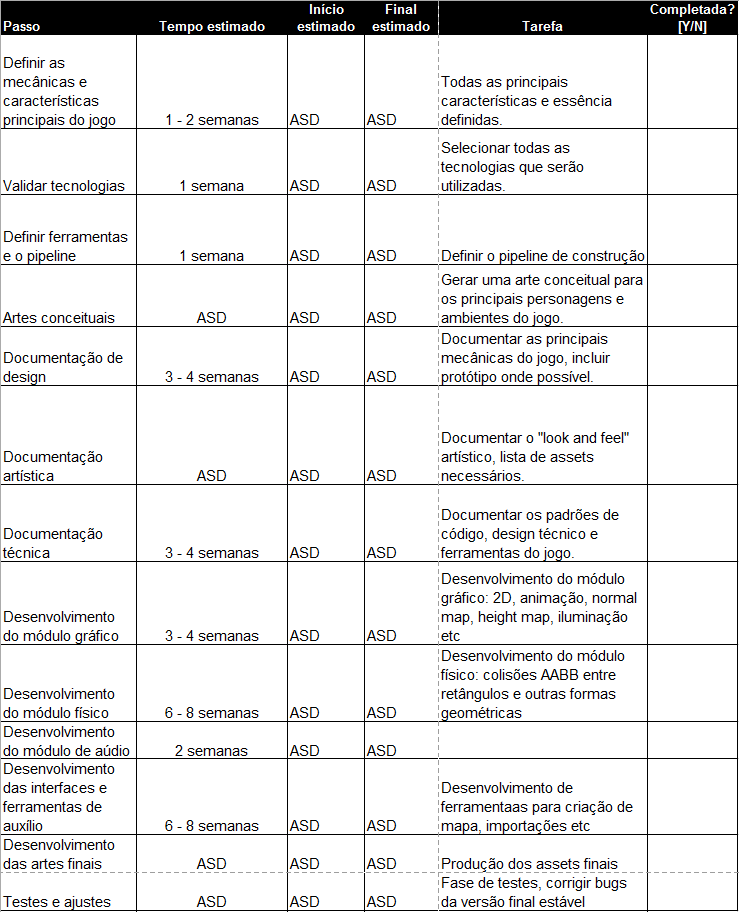
\includegraphics[width=4in]{imagens/cronograma.png}
	\caption{Tabela com uma estimativa de tempo para cada passo do desenvolvimento}
\end{figure}

% ------------------------------------------
% REFERENCIAL TEÓRICO

\chapter{Revisão Bibliográfica}

\section{Referencial Teórico}
\label{sec:refteo}
\subsection{OpenGL}
A API (Application Programming Interface) OpenGL fornece um conjunto de funções para manipulações gráficas \cite{LearnOpenGL}, sendo acelerada diretamente em hardware, multiplataforma, robusta e totalmente escalável. Embora comumente referida como uma API, o OpenGL é, por si só, um conjunto de especificações que determinam o resultado/saída de cada função e como devem ser executadas. Fica a cargo dos manufaturadores de placas gráficas implementarem a operação da função, respeitando as especificações do documento desenvolvido e mantido pela Khronos Group \cite{KhronosOpenGLSpecification}.
 O OpenGL foi lançado em 1992 como uma resposta direta a necessidade de se padronizar o conjunto de instruções usado em hardwares com interface gráfica. Até setembro de 2006 o padrão foi mantido pela ARB (Architecture Review Board), um conselho formado por empresas de grande renome no ramo como HP, IBM, Intel, NVIDIA, Dell e a própria fundadora, a Silicon Graphics. Em setembro de 2006 o conselho ARB tornou-se o OpenGL Working Group gerido e mantido pelo consórcio Khronos Group para Open Standard APIs\cite{OpenGLAbout}.
 
\subsection{Engenharia de software}
A engenharia de software em um jogo, para ser bem sucedida, precisa respeitar as etapas de pré-produção, produção, testes (ou Quality Assurance) e pós-produção [Manual de produção de jogos digitais – Pg. 3]. A metodologia de desenvolvimento a ser utilizada neste trabalho será o SCRUM.

\subsection{Pré-Produção}
A etapa de pré-produção é crítica e determina como será o jogo, quanto tempo levará o desenvolvimento, quantas pessoas serão necessárias e quanto irá custar tudo. Geralmente consome de 10 a 25\% do tempo total do desenvolvimento \cite{Manualdejogosdigitais}. É nessa etapa que se elabora o Game Design Document (GDD) contendo todo o conceito do jogo e requisitos do projeto.

\subsection{Produção}
Durante a produção será elaborado os assets e código do jogo. É nela que ocorrem a criação do conteúdo propriamente dito e o rastreamento do progresso e conclusão de tarefas\cite{Manualdejogosdigitais}. Para equipes pequenas é interessante metodologias ágeis que focam na produção invés de documentação.

\subsection{Testes}
Em jogos há duas grandes fases para verificar se tudo está funcionando como o esperado: Alfa e Beta. Durante todo o processo é necessário uma equipe do Departamento de Qualidade verificando bugs e reportando-os. Entretanto, as fases Alfa e Beta são as mais importantes. A fase alfa é quando uma seleta quantidade de usuários é escolhida para testar o jogo e dar feedback à desenvolvedora. Ela é fundamental para garantir que o jogo funciona como esperado e quais aspectos precisam ser melhorados antes de ser distribuída para o público geral. A etapa seguinte, Beta, é geralmente aberta ao público e já possui boa parte dos bugs corrigidos. Ela é essencial para testar a recepção do público e fazer as correções finais antes do lançamento oficial.

\subsection{Game Design Document}
Como em todo software o jogo também possui um documento de requisitos. Entretanto, um documento de requisitos não é suficiente para detalhar todos os elementos que compõe um jogo.  Essa carência de especificações como história, personagens, roteiro, câmera entre outras coisas são supridas pelo GDD.  Portanto, no caso especial de um jogo é necessário ambos documentos para detalhar e especificar adequadamente o projeto. Entretanto, não há regra universal ou normas que ditem como exatamente um GDD deve ser construído ou quais conteúdos deve abranger. A estrutura de um GDD é, possivelmente, composta dos seguintes itens \cite{LevelUp}:\\ %TODO: Citei apenas os mais relevates, isso altera a maneira de citar uma vez que não está idêntico ao do livro?
\textbf{Objetivos de jogo} – Detalha o conceito geral do jogo.\\
\textbf{Visão geral da história} – Constitui um breve resumo da história. Deve entrelaçar os diversos elementos narrativos como ambientes e personagens e conter o início, meio e fim da narrativa. \\
\textbf{Controles do jogo} – Lista de movimentos que o jogador poderá realizar como ataques, rolamento e corrida. Deve mapear cada botão do controle com a ação a ser realizada. \\
\textbf{Exigências de tecnologia} – Ferramentas que serão utilizadas ou implementadas para design de níveis, câmeras, engine, física etc. \\
\textbf{Front end do jogo} – Indica quais telas de crédito serão mostradas quando o jogo é ligado pela primeira vez incluindo: 
	\begin{itemize}
	\item Distribuidor
	\item Logo do estúdio
	\item Licenciadores
	\item Produtores de software terceirizados
	\item Tela com legislação
	\end{itemize}
\textbf{Tela de título/início} - Deve conter em detalhes o que é apresentado ao jogador nas telas iniciais, de preferência com imagens, como por exemplo: Título e como ele aparece na tela, tela de configurações (vídeo, áudio, música, subtítulos etc.), lista de detalhes dos arquivos salvos etc.\\
\textbf{Outras telas} - Todas as outras telas que não as de início. Por exemplo: Créditos, Conteúdos desbloqueáveis, easter eggs, roupas e armas alternativas etc.\\
\textbf{Fluxo de jogo} - Demonstra através de um fluxograma como todas as telas interagem entre si.\\
\textbf{Câmeras(s) de jogo} - Deve conter todos os tipos de câmeras utilizadas, sejam primeira pessoa, terceira pessoal, de rolagem etc.\\
\textbf{Sistema de HUD} - Informações apresentadas em tela para o jogador. Deve conter imagens demonstrados aspectos como: Saúde, Vidas, Dinheiro, Mini Mapa, Sistema de mira, Sistema de navegação, habilidades etc.\\
\textbf{Personagem do jogador} - Alguns conceitos visuais e textuais de quem é o personagem que o jogador irá controlar.\\
\textbf{Métricas do jogador} - Relações de tamanho do personagem do jogador com outros/elementos no mundo:
	\begin{itemize}
	\item Movimento (caminhada, corrida, movimento furtivo, mergulho,rolagem, rastejada)
	\item Navegação (nado, pulo, voo)
	\item Pendurar/Balançar
	\item Movimentos sensíveis ao contexto (empurrar/puxar, iterações com objetos etc.)
	\item Reações/danos/morte	
	\end{itemize}
\textbf{Habilidades do jogador} - Descrição de cada uma das habilidades e seus upgrades, modificadores e métricas.
\textbf{Mecânicas Universais de jogo} - Descrição breve de como cada uma das mecânicas que compõe o jogo funciona.
\textbf{Pontuação} - Métricas de como o jogador é recompensado. Placares de liderança e  Achievements.
\textbf{Economia} - Sistema monetário e o que é possível obter com a moeda. Lista custos.
\textbf{Veículos} - Como funcionam os veículos. Como interagir, suas métricas e controles.
\textbf{Personagens relevantes na história} - Um breve resumo de cada personagem importante para a história e o seu papel. Mostrar imagens.
\textbf{Esboço da progressão do jogo} - Mostrar em um esboço textual ou visual como seria jogar o jogo do começo ao fim. Deixe explicito como o jogador é recompensado conforme progride na história.   
\textbf{Regras gerais dos inimigos} - Listar:
	\begin{itemize}
	\item Tipos de comportamento (patrulheiro, caçador etc.)
	\item Regras de IA e métricas de detecção
	\item Parâmetros de nascimento
	\item Parâmetros de derrota etc.
	\end{itemize}
\textbf{Personagens não jogáveis (NPCs)} - Descrição breve dos tipos de NPC e listar possíveis características como nomes, onde encontrá-los, história etc. Determinar também as interações possíveis.\\
\textbf{MiniGames} - Lista quais minigames estão presentes bem como seus controles e onde aparecem.\\
\textbf{Cenas de corte} - Listar as cenas de corte.\\
\textbf{Músicas e efeitos especiais} - Listar as músicas e efeitos juntamente com seu tom/clima e onde aparecem.\\
\textbf{Apêndices} - Lista de animações do jogador, Lista de animações dos NPCs e inimigos, Lista dos efeitos sonoros, Lista de músicas, Roteiros etc.
% ------------------------------------------
% Trabalhos Correlatos

\chapter{Trabalhos Correlatos}
\label{sec:trabcorr}

%TODO: Inserir imagem
No Place for bravery: Jogo estilo Roguelike em pixel art. Atualmente em desenvolvimento pelo estúdio Glitch Factory situado no Distrito Federal.\\

%TODO: Inserir imagem
Eitr: Jogo estilo Action RPG inspirado em Dark souls com uma temática sombria e em pixel art. Atualmente em desenvolvimento pelo estúdio Devolver Digital.\\

%TODO: Inserir imagem
Kingdom: Jogo de plataforma feito em pixel art. \\

Moon Hunters: Action RPG em pixel art com mundo extenso e procedural, muito similar à proposta deste trabalho em alguns aspectos centrais. \\

Children of morta: Action RPG em pixel art. \\

% ------------------------------------------
% DESENVOLVIMENTO DO TRABALHO

\chapter{Arquitetura de uma game engine}
Game engine (em português literal, motor de jogo) é o termo designado ao motor que está por trás de todo jogo. É neste conjunto de sistemas de simulação em tempo real que todo o ambiente do jogo é construído. As principais funcionalidades providas em uma engine são um sistema de renderização 2D e/ou 3D, detecção e resolução de colisões, áudio e inteligência artificial. A partir desses elementos há várias ramificações em subsistemas com funcionalidades específicas para satisfazer as necessidades individuais de cada projeto. Uma engine se assemelha em muitas características a um sistema operacional. Ela lida com aspectos de baixo nível da máquina como a \textit{Graphic Processing Unit} (GPU) e é comummente construída utilizando-se o padrão de projeto em camadas. A Figura ~\ref{fig:arquitetura}  ilustra um típico diagrama da arquitetura desse sistema e seus componentes.

Alguns exemplos muito populares de engines disponíveis no mercado são a Unity, Unreal Engine, Godot, Construct 2 entre muitas outras. Cada uma apresenta sua própria estrutura e especificidade. Algumas são voltadas para projetos 3D e 2D, outras são otimizadas especificamente para um ambiente 2D e outras 3D. Cabe ao projetista decidir qual desses produtos irá melhor atende-lo conforme suas necessidades. Para este projeto, a engine utilizada será de desenvolvimento próprio.

\begin{figure}[H]
	\centering
	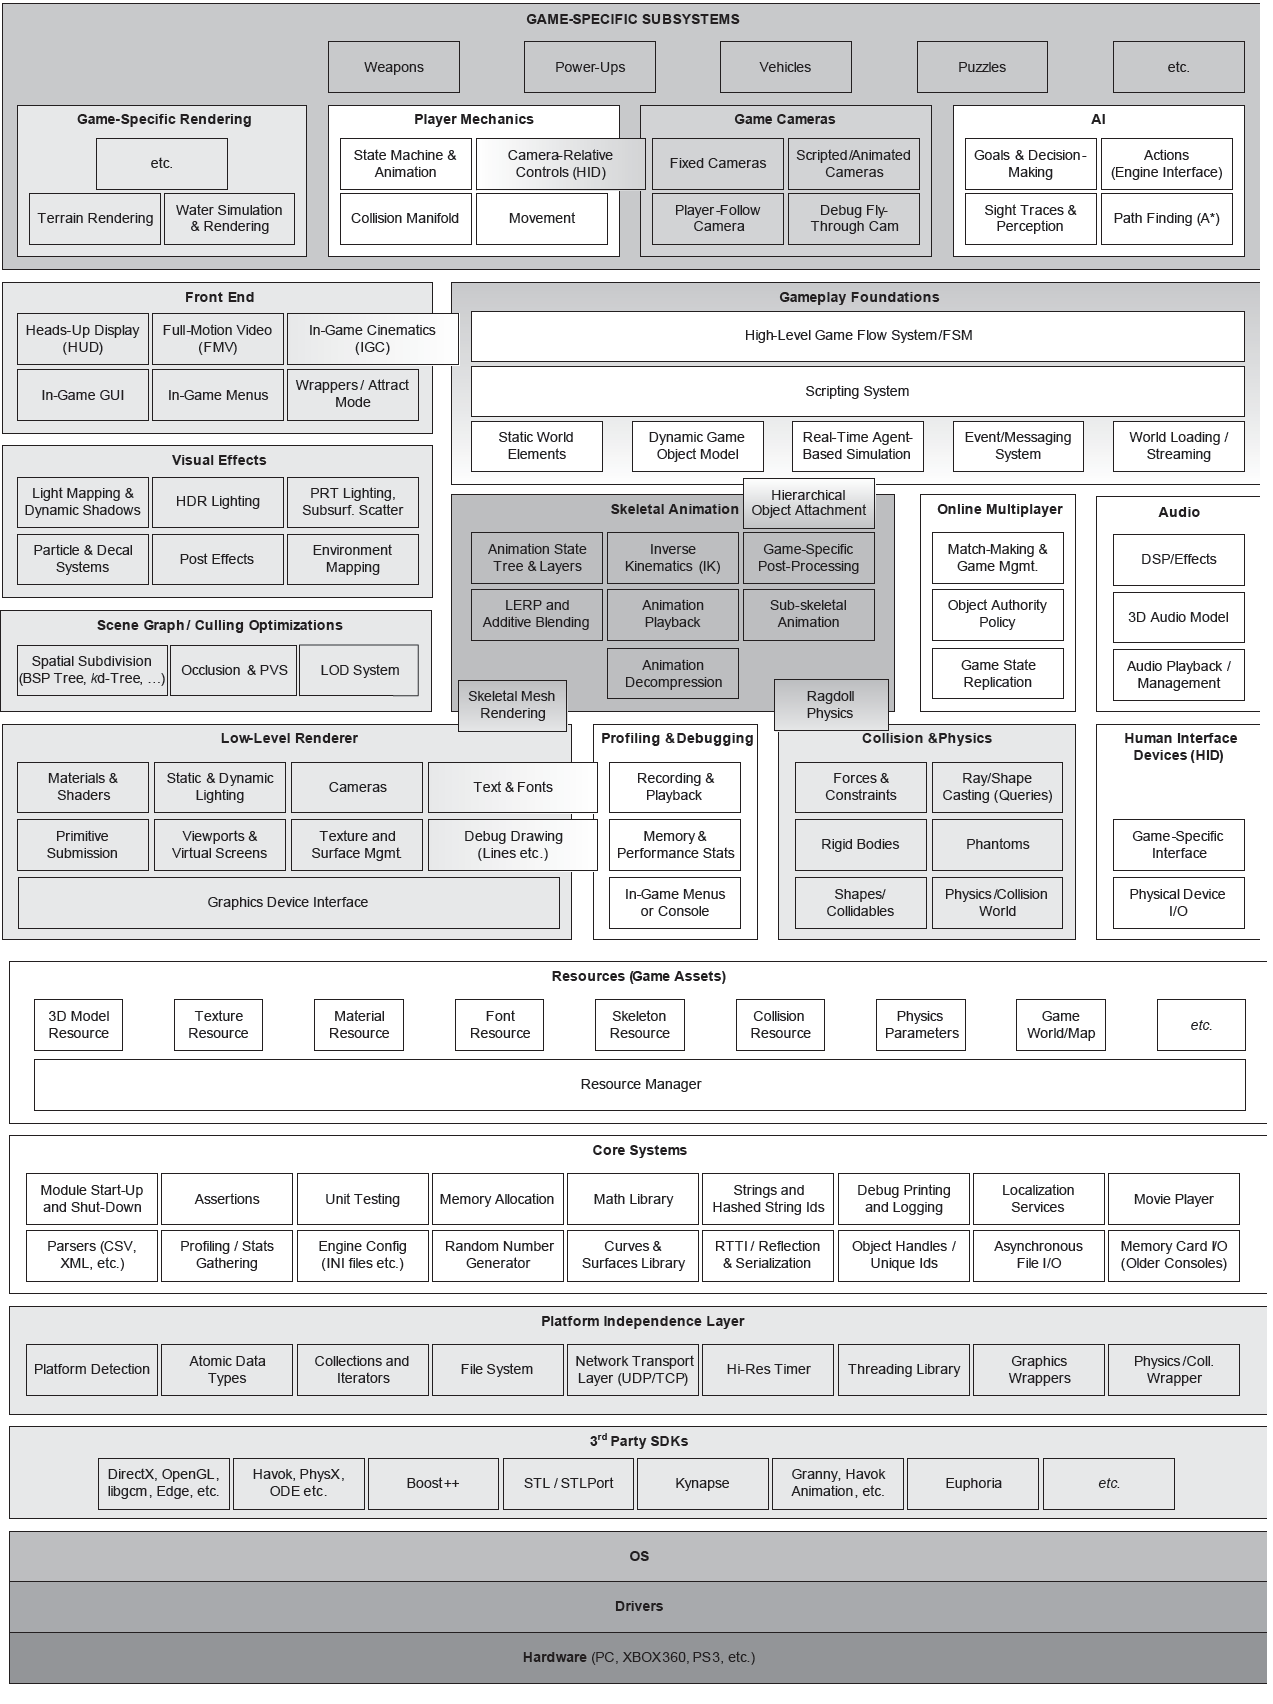
\includegraphics[width=\textwidth]{imagens/engine_layers.png}
	\caption{Componentes de uma Game Engine. Fonte:~\cite{GameEngineArchitecture}
    \label{fig:arquitetura}}
\end{figure}

\section{Game loop}
Game loop é o núcleo da arquitetura de uma engine. É neste loop que todos os subsistemas da engine são chamados e  executados, como a renderização, detecção e resolução de colisões, áudio e muitos outros \cite{GameEngineArchitecture}. Por se tratar de uma simulação em tempo real, onde a tela inteira deve ser atualizada em uma quantidade muito alta de vezes, é fundamental que tudo seja executado o mais rápido possível e em tempo constante para que o usuário tenha uma experiência fluída e dinâmica.\\
Portanto, o tempo demanda um papel chave neste sistema e deve ser cuidadosamente levado em consideração para que não haja quaisquer gargalos que deturpem a fluidez e experiência final do usuário. A estrutura mais simples de um game loop é composta como se segue:\\

\begin{lstlisting}[caption=Estrutura básica do Game Loop]
while(true) {
	update();
	render();
}
\end{lstlisting}
Esse código sendo executado ao longo do tempo é representado pela figura:
\begin{figure}[H]
	\centering
	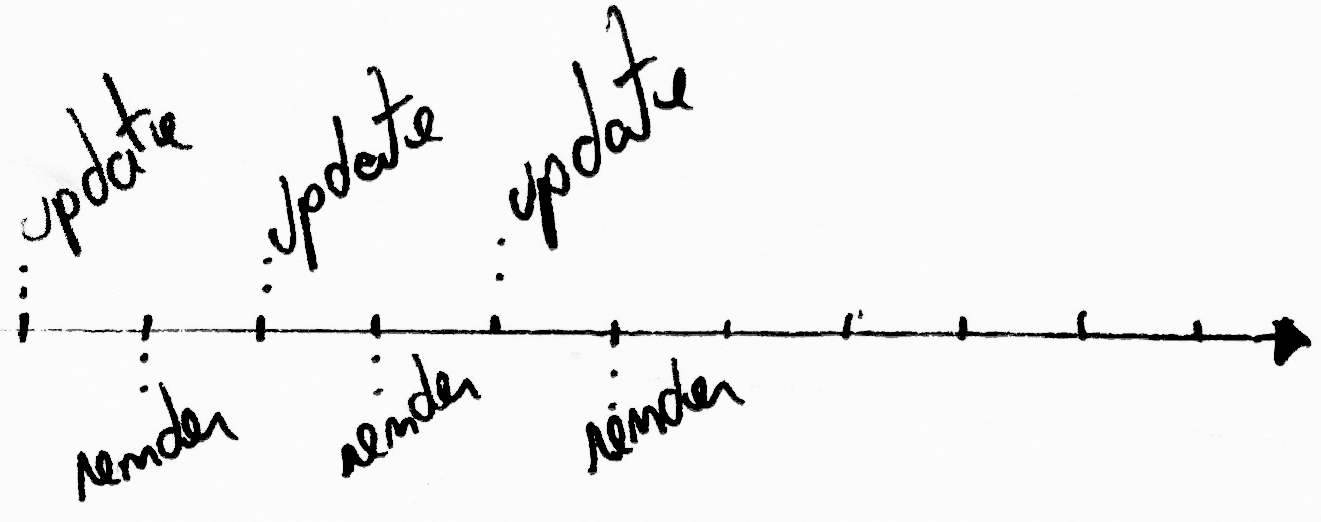
\includegraphics[width=\textwidth]{imagens/ilu1.png}
	\caption{Execução do game loop básico ao longo do tempo}
\end{figure}

Cada execução do método \texttt{render} significa o desenho de uma imagem na tela e a quantidade total de imagens desenhadas ao longo de um segundo é representado pela sigla FPS (\textit{Frames per second}). Cada execução do método \texttt{update} significa um passo no tempo do jogo (\textit{timestep}). Da mesma forma que o relógio move em tiques de um segundo em um segundo, o tempo do jogo move em tiques de \texttt{update} em \texttt{update}.


\section{Sistema de atualização}
O sistema de atualização é responsável por controlar o aspecto lógico da engine. Nele ocorre todos os cálculos relativos a movimentação dos objetos, colisões, inteligência artificial e outros. Sendo assim, é um sistema composto de outros sistemas, cada um rodando com uma taxa de atualização específica e não obrigatoriamente atrelados ao FPS.

\subsection{Timestep fixo}
Sistemas de atualização com timestep fixo são aqueles que estavam diretamente atrelados ao FPS e eram utilizados em jogos antigos \cite{GameEngineArchitecture}. As unidades de medida de tempo eram diretamente atreladas ao FPS tal que se uma máquina é capaz de rodar o jogo a 30 FPS e outra a 60 FPS, na segunda máquina o jogo daria impressão de estar duas vezes mais rápido ou duas vezes mais lento dependendo do valor fixado para o timestep. Isso acontecia por que os jogos eram desenvolvidos para plataformas específicas e, sabendo em qual taxa de FPS o jogo iria rodar, era fácil delimitar um timestep fixo para o jogo.

Entretanto, conforme as máquinas se tornaram mais potentes e o mercado passou a oferecer mais opções de hardware, logo a indústria estava produzindo jogos para um SO com múltiplas possibilidades de hardware. Essa gama de computadores com poderes de processamento distintos gerou o problema descrito acima. Por exemplo, defina-se uma máquina \texttt{MA} capaz de rodar o jogo a 30 FPS e uma máquina \texttt{MB} capaz de rodar a 60 FPS, sendo a máquina \texttt{MA} o alvo do projeto. Se um personagem deveria mover-se 300 pixels por segundo, logo 10 pixels por frame ($300 px/ 30 FPS$), na máquina \texttt{MB} ele estaria se movendo a 600 pixels por segundo pois ao dobrar o \textit{FPS} dobra-se a quantidade de vezes que chamamos o método \texttt{update} e portanto o personagem passa a mover-se 600 pixels por segundo ($60 FPS * 10 px$). Isso acontece por que antigamente o jogo era projetado para rodar numa máquina cuja capacidade de FPS seria $x$ e a variável $\Delta t$, que representa o tempo transcorrido entre um frame e outro, seria o inverso de $x$, ou simplesmente o inverso da frequência, o período $1/x$. A partir disso a posição do objeto era calculada efetuando-se $pos(i) = pos(i-1) + velPerFrame$ e como $\Delta t$ é um valor fixo dado por $1/x$ (baseado num FPS de $x$), tem-se que em um computador mais potente, o tempo transcorrido entre um frame e outro é menor e portanto o período aumenta. Como o valor foi pré calculado para uma máquina alvo ele não diminui na máquina mais potente e acaba sendo somado mais vezes, resultando em uma velocidade maior que a originalmente desejada. Esse problema pode ser facilmente representado por uma série.

Em um PC capaz de rodar a 30FPS: $$\sum_{n=1}^{30} 10px = 300 px/s$$
Em um PC capaz de rodar a 60FPS: $$\sum_{n=1}^{60} 10px = 600 px/s$$
Sendo assim, a estrutura do game loop com timestep fixo seria:
\begin{lstlisting}[caption=Game Loop com timestep fixo]
public static final float dt = 1f/30f;

while(true) {
	update(dt);
	render();
}
\end{lstlisting}
E pode ser representado pela figura:
\begin{figure}[H]
	\centering
	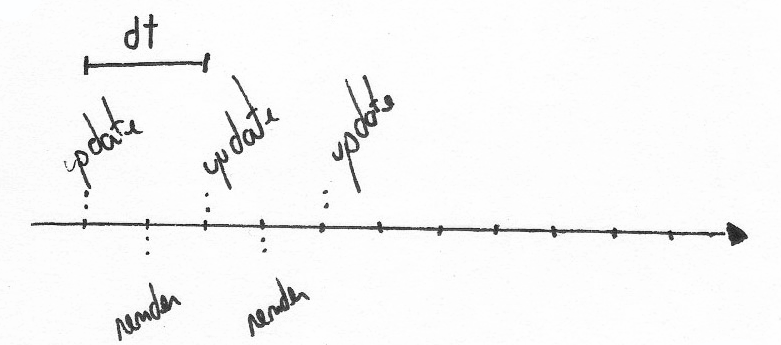
\includegraphics[width=\textwidth]{imagens/ilu2.png}
	\caption{Execução do game loop com timestep fixo ao longo do tempo}
\end{figure}
\subsection{Timestep variável}
Tornando a taxa de atualização $\Delta t$ dinâmica ao invés de fixa ela passa a ser independente do FPS. Isso é possível medindo quanto tempo se passou entre um frame e outro. Dessa forma o game loop fica:\\
\begin{lstlisting}[caption=Game loop com timestep variável]
private long lastFrame;
private long dt;
		
while(true) {
	long currentFrame = System.nanoTime(); 
	dt = currentFrame - lastFrame;
	lastFrame = currentFrame;
	
	update(dt);
	render();
}
\end{lstlisting}
Esse código é representado pela figura:
\\//TODO: Insert Ilu. 3\\

Embora tenha-se resolvido o problema anterior de dois computadores com poder de processamento diferente, o sistema ainda não é ideal. A falha está no fato de utilizar o $\Delta t$ anterior ao frame atual. Se o tempo passado entre um frame e outro for muito grande, ou seja, se tivermos um pico de performance, será avançado um tempo muito grande e um passo do personagem que era para ser $10 pixels$, passa a ser $10px + atraso$ e este efeito chamado de \textit{stuttering} é percetível ao jogador, pois atrapalha a fluidez da movimentação. Isso também traz consequências na lógica do programa. Um objeto que deveria percorrer 10 pixels por timestep, ao percorrer mais em um único timestep poderia, por exemplo, estar ignorando uma colisão que deveria ocorrer entre o ponto atual e o próximo.
\begin{figure}[H]
	\centering
	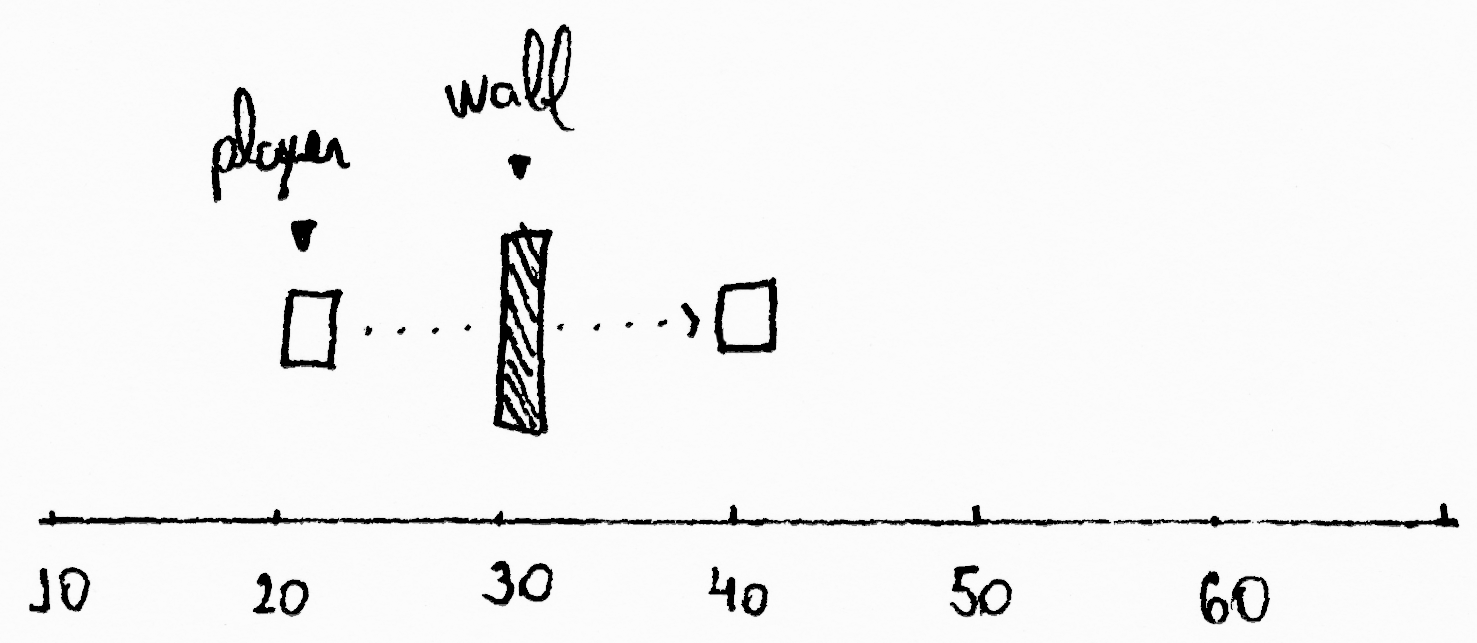
\includegraphics[width=\textwidth]{imagens/ilu4.png}
	\caption{Objeto ignorando colisão devido um timestep muito grande}
\end{figure}
 Não só isso, mas um timestep variável traz toda uma complicação com a depuração. Ao introduzir um fator não determinístico no processo, pode ser que seja impossível reproduzir um cenário de bug para efetuar seu diagnóstico e correção. 

\subsection{Timestep semi-fixo}
Um game loop com timestep semi-fixo tenta trazer o melhor dos dois mundos. Isso é possível usando um $\Delta t$ fixo para cada chamada do método update e, quando o sistema demorar mais que o $\Delta t$ fixado, faz-se a recuperação do mesmo chamando o método \texttt{update} quantas vezes necessário.
Isso é fácil visualizar quando demonstrado em código:
\begin{lstlisting}[caption=Game Loop com timestep semi-fixo]
private long lastFrame;
private long accumulator = 0;
private long dt;
public static final long ONE_SECOND_IN_NANOSECONDS = 10^9;
public static final long STEPS_PER_SECOND = 30;
public static final long FIXED_DT = ONE_SECOND_IN_NANO/STEPS_PER_SECOND;
			
while(true) {
	long currentFrame = System.nanoTime(); 
	dt = currentFrame - lastFrame;
	lastFrame = currentFrame;
	accumulator += dt;
	
	while (accumulator >= FIXED_DT){
    	update(dt);
    	accumulator -= FIXED_DT;
 	 }
 			 
	render();
}
\end{lstlisting}
É importante ter cuidado com o valor escolhido para o \texttt{FIXED_DT}(timestep). Se o timestep for menor que o tempo que se leva para processar o método \texttt{update} o sistema nunca irá recuperar seu atraso, tendo um acumulador que sempre cresce e nunca fica próximo de zerar \cite{GameProgrammingPatterns}.
O sistema de timestep semi-fixo é demonstrado pela ilustração:
\\//TODO: Insert Ilu. 6
 
\section{Sistema de renderização}
É neste sistema que todos os objetos visíveis na tela são desenhados. Esse sistema é executado diversas vezes e em rápida sucessão durante um segundo, criando uma ilusão de movimento. Esse processo se inicia no processador e termina na placa gráfica acontecendo quantas vezes a máquina conseguir ou quantas vezes o usuário desejar configurar. Os valores mais comuns são atrelados à frequência do monitor que, atualmente, variam de 30 Hz até 144 Hz e para todos os efeitos são o equivalente ao FPS \cite{GameEngineArchitecture}.

\subsection{Interpolação Linear} 
Com o timestep definido ainda é necessário mais um procedimento para que o sistema renderize objetos em movimento de forma suave. O efeito de \textit{stuttering} pode ser causado tanto pelo aspecto lógico, através dos picos de performance, quanto pelo simples fato de que não se possui controle total sobre o SO. Não é possível garantir uma taxa de atualização e renderização intercalada e perfeita. Haverá momentos que depois de um único \texttt{update} o método \texttt{render} será chamado várias vezes e, sem nenhum tratamento, este efeito também causa \textit{stuttering}. Ao chamarmos o método \texttt{render} consecutivamente e não atualizarmos a posição do objeto em cada chamada, para o usuário a impressão é de um sistema engasgado com um movimento não fluído.
Para resolver este último problema é necessário realizar uma interpolação linear entre a posição anterior e atual do objeto, tornando seu movimento suave. Esse efeito pode ser visualizado nas figuras a seguir onde um objeto move-se 10 pixels por segundo. Na primeira figura a função \texttt{render} é chamada sem nenhum tratamento e portanto renderiza o objeto no mesmo lugar até que sua posição seja atualizada no próximo \texttt{update}. Já na segunda figura, é renderizado a interpolação da posição desse objeto, tornando seu movimento muito mais suave para o usuário.
\\//TODO: Insert Ilu 7
\\//TODO: Insert Ilu 5\\
E o código final do game loop com interpolação linear fica como se segue:
\begin{lstlisting}[caption=Game Loop com timestep semi-fixo e interpolação linear]
		long lastFrame;
		long accumulator = 0;
		long dt;
		public static final long ONE_SECOND_IN_NANOSECONDS = 10^9;
		public static final long STEPS_PER_SECOND = 30;
		public static final long FIXED_DT = ONE_SECOND_IN_NANO/STEPS_PER_SECOND;
		
		
		while(true) {
			long currentFrame = System.nanoTime(); 
			dt = currentFrame - lastFrame;
			lastFrame = currentFrame;
			accumulator += dt;
	
			while (accumulator >= FIXED_DT){
    			update(dt);
    			accumulator -= FIXED_DT;
 			 }
 			 
			long interpolationFactor = accumulator / FIXED_DT; 			 
 			 
			render(interpolationFactor);
		}
\end{lstlisting}
Dentro da função \texttt{render} o fator de interpolação é utilizado na seguinte fórmula para obter a posição onde o objeto deve ser renderizado:

\begin{quote}
$renderPosition$ = $currentPosition * interpolationFactor$ + $previousPosition * (1 - interpolationFactor)$
\end{quote}

\section{API gráfica OpenGL}
OpenGL é a API encarregada pela comunicação com a GPU. Através dela são realizadas todas as chamadas de função responsáveis por desenhar objetos na tela. Cada Engine deve utilizar uma API dependendo da plataforma na qual o produto final será disponibilizado. Por exemplo, para um sistema mobile existe a API OpenGL ES, para windows tem-se a OpenGL, DirectX etc. De certa forma, as APIs gráficas por si só são aquilo que na essência compõem o sistema de renderização.  
\subsection{Core-profile e Immediate mode}
Immediate mode (legacy) é o modo antigo de se operar com OpenGL. Hoje ele é depreciado e substituído pelo modo Core-profile. No modo antigo as funções eram mais fáceis de usar, com muitas da funcionalidades já abstraídas pela API. Entretanto, por serem abstraídas elas forneciam uma menor flexibilidade de controle sobre como o OpenGL  operava e eram também ineficientes\cite{LearnOpenGL}. Com o passar do tempo e uma demanda dos desenvolvedores por maior flexibilidade a API foi depreciada e substituída pelo modo Core-profile, nele tem-se muito mais controle sobre como o OpenGL opera. Entretanto, isso vem ao custo de uma maior curva de aprendizagem e complexidade de implementação.
\subsection{State Machine}
O OpenGL funciona como uma enorme máquina de estados, possuindo uma enorme coleção de variáveis que definem como  operar no estado vigente. Chama-se as funções para configurar o estado atual, passando buffers e outras informações para então renderizar o estado atual.

\subsection{Hello window}
A primeira peça necessária para usar o OpenGL é criar um contexto e uma janela onde renderizar. O processo de criação da janela é especifico de cada SO e faz-se necessário uso de outra API para abstrair esse passo. Neste documento será utilizado a biblioteca \texttt{GLFW}. O código a seguir demonstra esse processo e é explicado a seguir:
\begin{lstlisting}[caption=Inicialização da janela e contexto OpenGL]
public void init() {
	if (!glfwInit()) 
		System.err.println("Could not initialize GLFW.");

	glfwWindowHint(GLFW_CONTEXT_VERSION_MAJOR, 3);
	glfwWindowHint(GLFW_CONTEXT_VERSION_MINOR, 3);
	glfwWindowHint(GLFW_OPENGL_PROFILE, GLFW_OPENGL_CORE_PROFILE);
	glfwWindowHint(GLFW_RESIZABLE, GL_FALSE);

	id = glfwCreateWindow(width, height, name,  NULL,  NULL);
	glfwMakeContextCurrent(id);

	glfwSetWindowPos(id, 2000, 60);
	glfwShowWindow(id);
	GL.createCapabilities();
	glfwSwapInterval(1); //VSYNC

	glViewport(0,0, width, height);
	glEnable(GL_CULL_FACE);
	glEnable(GL_BLEND);
	glBlendFunc(GL_SRC_ALPHA, GL_ONE_MINUS_SRC_ALPHA);
}
\end{lstlisting}
Primeiramente inicializa-se o GLFW chamando \texttt{glfwInit}. Em seguida usa-se a função \texttt{glfwWindowHint} para adicionar atributos a janela, sendo o primeiro argumento o nome do atributo e o segundo argumento o valor que se deseja atribuir. Aqui foram inseridos os atributos \texttt{GLFW_CONTEXT_VERSION_MAJOR} e \texttt{GLFW_CONTEXT_VERSION_MINOR} para indicar qual a versão ideal e mínima para rodar a aplicação. No caso essa versão é a 3.3. O atributo \texttt{GLFW_OPENGL_PROFILE} altera entre o modo core profile e immediate mode (Legacy). Cria-se então a janela com o método \texttt{glfwCreateWindow} e usa-se o id retornado para torná-lo o contexto vigente com \texttt{glfwMakeContextCurrent}. A função \texttt{glfwShowWindow} é chamada para tornar essa janela visível ao usuário. Para utilizar o OpenGL e criar seu contexto é necessário chamar \texttt{GL.createCapabilities}. A partir deste ponto o OpenGL pode ser utilizado normalmente.

\subsection{OpenGL pipeline}
A fim de poder desenhar objetos na janela é necessário abordar os \textit{buffer objects} e \textit{pipeline} presentes no OpenGL. Os \textit{buffer objects} são estruturas responsáveis por transmitir e receber dados da GPU. Existem 9 tipos de objetos e estes são divididos em duas categorias:
\\ \textbf{Regular objects}
\\ Objetos dessa categoria contem dados.
\begin{itemize}
\item Buffer object
\item RenderBuffer object
\item Texture object
\item Query object
\item Sampler object
\end{itemize}
\textbf{Container objects}
\\ Objetos dessa categoria servem apenas de containers para transportar os elementos da lista anterior. (\textit{regular objects}). 
\begin{itemize}
\item Framebuffer object
\item Vertex Array object
\item Transform Feedback object
\item Program pipeline object
\end{itemize}

Neste primeiro momento será abordado o \textit{Vertex Buffer Object} (VBO) e \textit{Vertex Array Object} (VAO). A fim de desenhar um objeto na tela faz-se necessário enviar a GPU os vértices que o compõem. O \textit{pipeline} recebe como entrada uma série de vértices 3D, os processa e transforma em pixels 2D na tela \cite{LearnOpenGL}. Cada etapa do \textit{pipeline} recebe como entrada a saída da etapa anterior.

As etapas customizáveis do \textit{pipeline} são processadas por pequenos programas chamados \textit{shaders}. Esses programas são escritos em GLSL pelo desenvolvedor da aplicação e ficam alojados na GPU, sendo altamente paralelizáveis e especializados. A seguir tem-se uma representação simplificada do processo que ocorre no pipeline.

\begin{figure}[H]
	\centering
	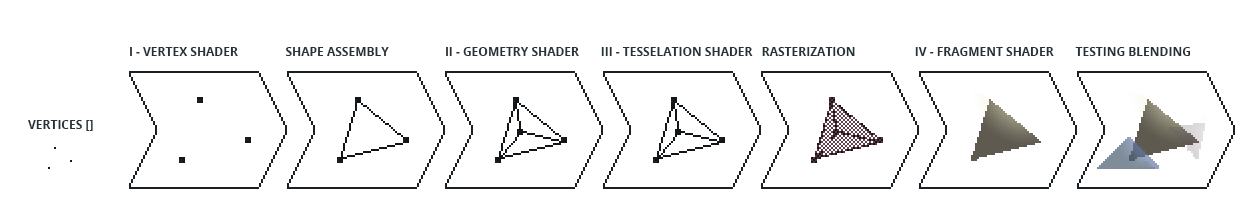
\includegraphics[width=\textwidth]{imagens/openglpipeline.png}
	\caption{Etapas do pipeline  \label{fig:pipeline}}
\end{figure}

Na etapa I o \textit{vertex shader} é responsável, principalmente, por receber um único vértice e processar sua coordenada cartesiana de um sistema para outro. Por exemplo, as coordenadas finais desse objeto vão mudar conforme a câmera se movimento no espaço. É também necessário converter a posição local do objeto para a sua posição global no ambiente. Esses e outros processos serão melhor abordados no capítulo sobre Sistemas de Coordenadas.

Na etapa do \textit{shape assembly} o OpenGL monta todos os vértices recebidos como entrada na primitiva selecionada para renderização. São algumas delas: \textit{GL_POINTS}, \textit{GL_LINES} e \textit{GL_TRIANGLES}.

A etapa do \textit{geometry shader} recebe como entrada a primitiva de saída do \textit{shape assembly}. A partir desses vértices o \textit{geometry shader} é capaz de gerar novos vértices e formar novas primitivas. No exemplo da figura \ref{fig:pipeline} ele recebe um triângulo e cria um novo vértice no centro, resultando em 3 sub triângulos.

O \textit{tesselation shader} é altamente especializado em subdividir uma primitiva em outras muito menores. Essa função é útil para, por exemplo, detalhar objetos mais próximos da tela e generalizar objetos mais distantes reduzindo sua quantidade de vértices.

A etapa de \textit{rasterization} processa a saída do \textit{tesselation shader} e converte todas essas informações em coordenadas 2D na tela ou, simplesmente, em pixels na tela. Esses pixels são então repassados como fragmentos para o \textit{fragment shader}.

Na penúltima etapa do pipeline, o \textit{fragment shader} processa todos os fragmentos para dar aos pixels sua cor final. É neste estágio que todos os efeitos visuais são aplicados como por exemplo a iluminação.

Por fim, no último estágio é aplicado o \textit{blending} e  outros testes. \textit{Blending} nada mais é do que calcular o quanto a transparência de um objeto afeta outro. No exemplo da figura \ref{fig:pipeline} isso é representado pelos dois triângulos menores que afetam a cor final do triângulo maior aonde estes se sobrepõem. Neste estágio também são realizados os testes de \textit{depth} e \textit{stencil}.

\subsection{Vertex Array Object e Vertex Buffer Object}
Todo objeto no OpenGL é manipulado através de seu ID. Portanto, faz-se necessário gerar o ID do VAO e VBO chamando as funções \texttt{glGenVertexArrays()} e \texttt{glGenBuffers()}. Após gerados os IDs vincula-se esse \textit{data object} como o vigente através da função \texttt{glBindBuffer(type , id)} e insere-se os dados nele através da função \texttt{glBufferData(type, data, draw_type)}. Para o \textit{object container} o processo é similar. Vincula-se o VAO com \textit{glBindVertexArray()} e habilita-se a localização do atributo do vértice no \textit{vertex shader} através da função \textit{glEnableVertexAttribArray()}. Por fim, configura-se como cada vértice deve ser interpretado, nesta situação como um bloco de 4 floats, sendo 2 deles as posições x e y do objeto e os dois últimos a posição x e y da textura que compõem esse objeto. Essa configuração é feita pela função \texttt{glVertexAttribPointer()}.

\begin{lstlisting}[caption=Inicialização do VBO e VAO]
private void init() {
	float vertices [] = {
			//Pos	//Texture
			0,	1,	0,	1f,
			1,	0,	1f,	0,
			0,	0,	0,	0,
			
			0,	1,	0,	1f,
			1,	1,	1f,	1f,
			1,	0,	1f,	0
	};
	
	int quadVAO = glGenVertexArrays();
	int VBO = glGenBuffers();
	
	glBindBuffer(GL_ARRAY_BUFFER, VBO);
	glBufferData(GL_ARRAY_BUFFER, BufferUtilities.createFloatBuffer(getVertices(3)), GL_STATIC_DRAW); 
	
	glBindVertexArray(quadVAO);
	glEnableVertexAttribArray(0);
	glVertexAttribPointer(0 , 4, GL_FLOAT, false, Float.BYTES * 4, 0);
	
	glBindBuffer(GL_ARRAY_BUFFER, 0);
	glBindVertexArray(0);
}
\end{lstlisting}

\subsection{OpenGL Shading Language (GLSL)}

\chapter{Desenvolvimento do trabalho}
\label{sec:desenv}
\section{Mecânicas}
\subsection{Sistema de caça ativa}
\begin{figure}[H]
	\centering
	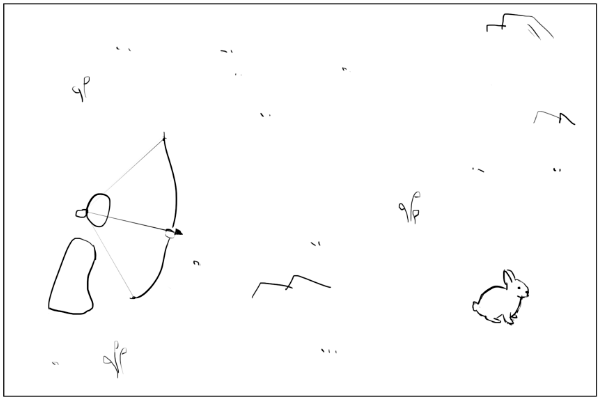
\includegraphics[width=4in]{imagens/mecanica_caca.png}
	\caption{Jogador caçando um coelho com arco e flecha}
\end{figure}
O sistema de caça é dado pelo seguinte fluxo de ações:
\begin{enumerate}  
\item Jogador avista animal em ambiente selvagem 
\item Ao se aproximar o animal pode perceber sua presença. Caso seja notado, a presa irá executar uma animação indicando que está desconfiado.
\item Se o jogador continuar avançando o animal irá tentar fugir 
\item Senão o jogador executa um ataque quando estiver ao alcance 
\end{enumerate}


\subsection{Sistema de armadilhas}
\begin{figure}[H]
	\centering
	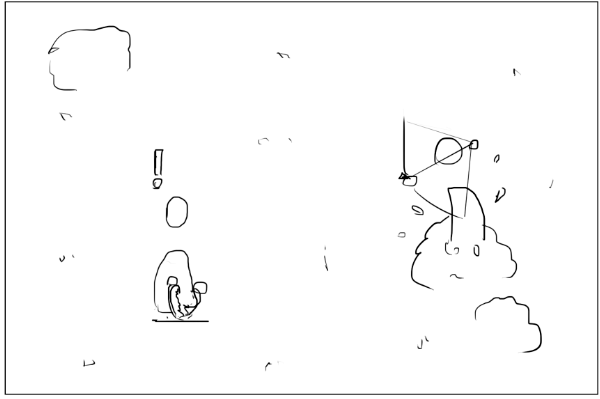
\includegraphics[width=4in]{imagens/mecanica_armadilha.png}
	\caption{Jogador pronto para atacar alvo que ficou preso na armadilha de chão}
\end{figure}
O sistema de armadilhas é dado pelo seguinte fluxo de ações:
\begin{enumerate}  
\item Jogador aciona armadilha no local desejado
\item Qualquer animal ou inimigo pode acionar a armadilha e acionar o seu efeito
\end{enumerate}

\subsection{Sistema de Combate}
O sistema de combate é delimitado pela arma escolhida. Cada arma implica em um estilo
de combate totalmente diferente e só pode ser utilizada ao aprender esse estilo com um
mestre. Os mestres podem ser encontrados aleatoriamente pelo mapa em grandes cidades de 
cada reino.

\subsection{Sistema de apadrinhamento}
Ao atingir um nível significante de reputação o jogador pode tentar ganhar um apadrinhamento de um rei ou lorde. Ganhando assim uma quantia semanal e benefícios como alimento e teto para poder compor suas músicas.

\subsection{Cantar músicas}
\begin{figure}[H]
	\centering
	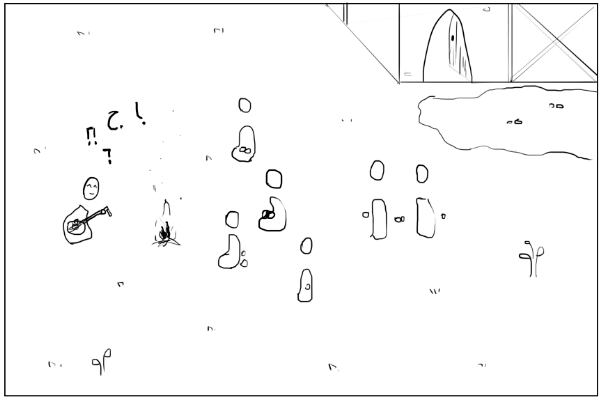
\includegraphics[width=4in]{imagens/mecanica_cantar.png}
	\caption{Jogador cantando em um vilarejo}
\end{figure}
\begin{figure}[H]
	\centering
	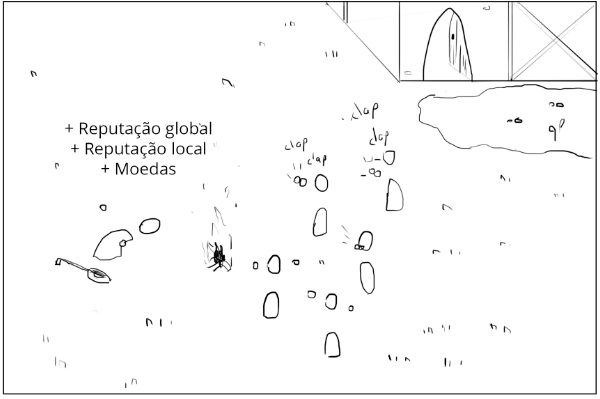
\includegraphics[width=4in]{imagens/mecanica_cantar2.png}
	\caption{Jogador sendo prestigiado após término da música}
\end{figure}
Cada vilarejo ou cidade tem um nível de interesse próprio em determinados instrumentos.
Quanto maior o interesse, maior serão as chances de receber uma boa quantia em ouro
pela apresentação.
As músicas podem ser tocadas em fogueiras que o próprio jogador pode criar em volta da cidade, ou em tavernas, festivais e praças.
\subsection{Compor músicas}
\begin{figure}[H]
	\centering
	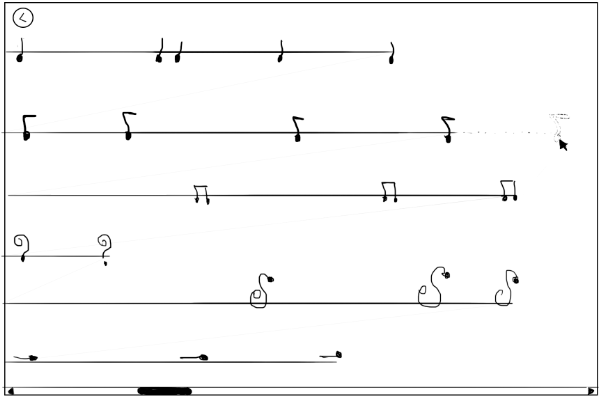
\includegraphics[width=4in]{imagens/mecanica_compormusica.png}
	\caption{Esboço do menu para compor músicas}
\end{figure}
ASD.
\subsection{Contar histórias}
ASD.
\subsection{Compor histórias}
ASD.
\subsection{Atributos dos vilarejos e cidades}
Cada cidade e vilarejo possui os seguintes atributos:
\begin{description}  
\item [Lista de interesses instrumentais] Cada vilarejo tem uma preferência por um instrumento. Quanto maior o interesse, maior a recompensa dada ao tocar músicas com aquele instrumento.
\end{description}

\subsection{Atributos do jogador}
\begin{description}  
\item [Fome] Ao longo do tempo o jogador precisa se alimentar para manter-se vivo. A fome é dividida em três estágios: Sem fome, fome controlável e faminto. Cada um dos estágios é
apresentado ao jogador em forma de uma animação de andar diferente. Quanto mais faminto o personagem está mais lento e curvado ele irá andar, até que ela chegue em zero e culmine na morte do personagem.
\end{description}

\subsection{Domar animais}
Alguns animais podem ser domados através dos instrumentos. Basta cantar próximo a eles então eles serão domados.

% ------------------------------------------
% EXPERIMENTOS E RESULTADOS
\chapter{Experimentos e resultados}
\label{sec:experim}








% ------------------------------------------
% CONCLUSÃO

\chapter{Conclusão}
\label{sec:conclus}







% ----------------------------------------------------------
% ELEMENTOS PÓS-TEXTUAIS


% ----------------------------------------------------------
\postextual

% ----------------------------------------------------------
% Referências bibliográficas
% ------------------------------------------
% REFERÊNCIAS MODELO DA FACOM
\bibliography{referencias}


% OS COMENTÁRIOS ABAIXO É CASO O TRABALHO TENHA ALGUM APÊNDICE
%% Apêndices TCC: só mantenha se for pertinente.
%% ----------------------------------------------------------

% ---
% Inicia os apêndices
% ---
%\begin{apendicesenv}

% Imprime uma página indicando o início dos apêndices
%\partapendices

% ----------------------------------------------------------
%\chapter{Quisque libero justo}
% ----------------------------------------------------------

%\lipsum[50]

% ----------------------------------------------------------
%\chapter{Coisas que fiz e que achei interessante mas não tanto para entrar no corpo do texto}
% ----------------------------------------------------------
%\lipsum[55-57]

%\end{apendicesenv}
% ---


% ----------------------------------------------------------
% Anexos %TCC: so mantenha se pertinente.
% ----------------------------------------------------------

% ---
% Inicia os anexos
% ---
%\begin{anexosenv}

% Imprime uma página indicando o início dos anexos
%\partanexos

% ---
%\chapter{Eu sempre quis aprender latim}
% ---
%\lipsum[30]

% ---
%\chapter{Coisas que eu não fiz mas que achei interessante o suficiente para colocar aqui}
% ---

%\lipsum[31]

% ---
%\chapter{Fusce facilisis lacinia dui}
% ---

%\lipsum[32]

%\end{anexosenv}

%---------------------------------------------------------------------
% INDICE REMISSIVO
%---------------------------------------------------------------------

\printindex



\end{document}